We provide intuition connecting hyperbolic space and tree distances, discuss the metrics used to measure embedding fidelity, and provide the relationship between reconstruction and learning for graph embeddings.


\begin{figure}
\centering
\begin{minipage}[b]{0.35\textwidth}
\begin{tikzpicture}[scale=2.0]
\tkzDefPoint(0,0){O}
\tkzDefPoint(1,0){A}
\tkzDefPoint(-1,0){B}
\tkzDefPoint(0.7071,0.7071){C}
\tkzDefPoint(-0.7071,-0.7071){Cn}
\tkzDefPoint(-.2,0.9798){R}
\tkzDefPoint(.2,-0.9798){Rn}
\tkzDrawCircle(O,A)

\tkzDefPoint(0.7,0.3){a}
\tkzDefPoint(0.8,0.1){b}
\tkzDefPoint(-.5,.5){w1}
\tkzDefPoint(-0.1,.9){v1}
 
\tkzDefPoint(-.6,.4){w2}
\tkzDefPoint(0,.95){v2}

\tkzDefPoint(-.7,.3){w3}
\tkzDefPoint(.1,.9){v3}
 
\tkzDefPoint(-.8,.2){w4}
\tkzDefPoint(.2,.85){v4}
 

\tkzDefPoint(0.2,0){t1}
\tkzDefPoint(0.4,0){t2}
\tkzDefPoint(0.6,0){t3}
\tkzDefPoint(0.8,0){x}
 
\tkzDefPoint(0.1414, 0.1414){u1}
\tkzDefPoint(0.2828, 0.2828){u2}
\tkzDefPoint(0.4243, 0.4243){u3}
\tkzDefPoint(0.5657, 0.5657){y}

 
\tkzClipCircle(O,A)
\tkzDrawCircle[orthogonal through=u1 and t1](O,A)
\tkzDrawCircle[orthogonal through=u2 and t2](O,A)
\tkzDrawCircle[orthogonal through=u3 and t3](O,A)
\tkzDrawCircle[orthogonal through=x and y](O,A) 
\tkzDrawPoints[color=black,fill=black,size=12](t1,t2,t3,y,u1,u2,u3,x)

  
\tkzDrawPoints[color=black,fill=black,size=12](O)
\tkzDrawLine[through=O](R,Rn) 
\tkzLabelPoints[right](y)
\tkzLabelPoints[above](x)
\tkzLabelPoints[above left](O)
    
\end{tikzpicture}
  \end{minipage}
  \begin{minipage}[b]{0.50\textwidth}
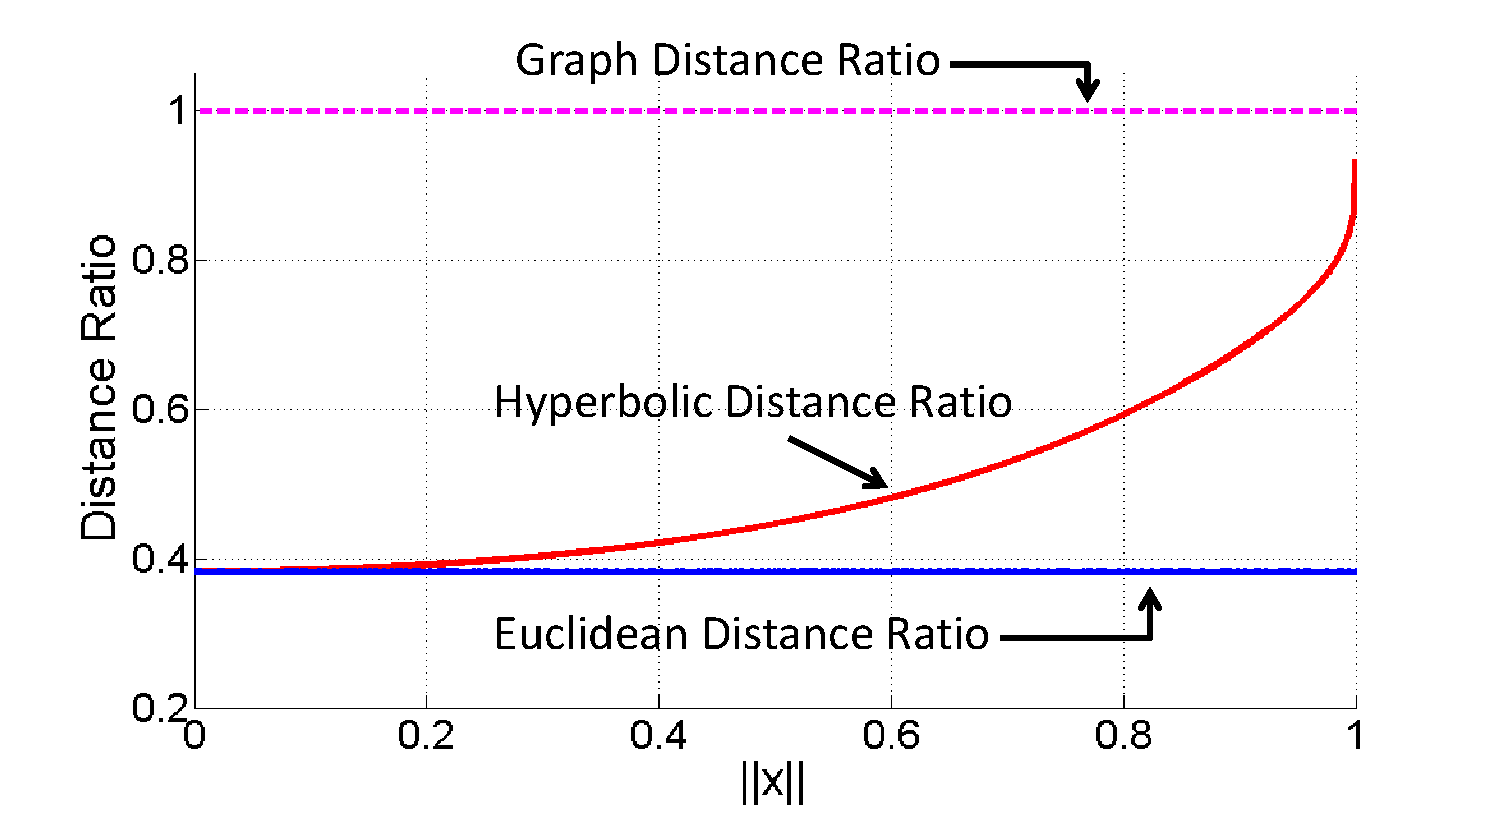
\includegraphics[width=0.9\textwidth]{figures/hyp_dist_4.pdf}
  \end{minipage}
\caption{Geodesics and distances in the Poincar\'{e} disk. As $x$ and $y$ move towards the outside of the disk (i.e., letting $\|x\|, \|y\| \rightarrow 1$), the distance $d_H(x,y)$ approaches $d_H(x,O)+d_H(O,y)$.} %Right: circle inversion takes $X$ to $X'$.}
\label{fig:geod}
\end{figure}

\paragraph*{Hyperbolic spaces} The Poincar\'{e} disk $\mathbb{H}_2$ is a
two-dimensional model of hyperbolic geometry with points located in
the interior of the unit disk, as shown in Figure~\ref{fig:geod}. A
natural generalization of $\mathbb{H}_2$ is the Poincar\'{e} ball
$\mathbb{H}_r$, with elements inside the unit ball. The Poincar\'{e}
models offer several useful properties, chief among which is mapping
conformally to Euclidean space. That is, angles are preserved between
hyperbolic and Euclidean space. Distances, on the other hand, are not
preserved, but are given by
\[d_{H}(x,y) = \text{acosh} \left( 1 + 2 \frac{\lVert { x}-{ y} \rVert^2}{(1-\lVert { x}\rVert^2)(1-\lVert { y}\rVert^2)} \right).\]

There are some potentially unexpected consequences of this formula,
and a simple example gives intuition about a key technical property
that allows hyperbolic space to embed trees. Consider three
points: the origin $0$, and points $x$ and $y$ with $\|x\|=\|y\| = t$ for some
$t > 0$. As shown on the right of Figure~\ref{fig:geod}, as
$t\rightarrow1$ (i.e., the points move towards the outside of the
disk), in flat Euclidean space, the ratio
$\frac{d_E(x,y)}{d_E(x,0)+d_E(0,y)}$ is {\em constant} with respect to
$t$ (blue curve). In contrast, the ratio $\frac{d_H(x,y)}{d_H(x,0)+d_H(0,y)}$ approaches 1, or, equivalently, the distance $d_H(x,y)$ approaches
$d_H(x,0)+d_H(0,y)$ (red and pink curves). That is, the shortest path between $x$ and $y$ is
almost the same as the path through the origin. This is analogous to the property of trees
in which the shortest path between two sibling nodes is the path through their parent.
This tree-like nature of hyperbolic space is the key property exploited by embeddings. Moreover,
this property holds for arbitrarily small angles between $x$ and
$y$.

\paragraph*{Lines and geodesics}  There are two types of geodesics (shortest
paths) in the Poincar{\'e} disk model of hyperbolic space: segments of circles that are orthogonal to
the disk surface, and disk diameters \cite{GeometryText}. Our algorithms and
proofs make use of a simple geometric fact: {\em isometric} reflection across geodesics
(preserving hyperbolic distances) is represented in this Euclidean model as a \emph{circle inversion}.
A particularly important reflection associated with each point $x$ is the one that takes $x$ to the
origin \citep[p.~268]{GeometryText}.

\paragraph*{Embeddings and fidelity measures} An \emph{embedding} is a mapping $f: U \rightarrow V$ for spaces $U,V$ with distances $d_U, d_V$. We measure the quality of embeddings with several \emph{fidelity measures}, presented here from most local to most global.

Recent work \cite{fb} proposes using the \emph{mean average precision} (MAP). For a graph $G=(V,E)$, let $a \in V$ have neighborhood $\mathcal{N}_a = \{b_1, b_2, \ldots, b_{\operatorname{deg}(a)}\}$, where $\operatorname{deg}(a)$ denotes the degree of $a$. In the embedding $f$, consider the points closest to $f(a)$, and define $R_{a,b_i}$ to be the smallest set of such points that contains $b_i$ (that is, $R_{a,b_i}$ is the smallest set of nearest points required to retrieve the $i$th neighbor of $a$ in $f$). Then, the MAP is defined to be
\[
\text{MAP}(f) 
=
\frac{1}{|V|}\sum_{a \in V} \frac{1}{|\mathcal{N}_a|}\sum_{i=1}^{|\mathcal{N}_a|} \text{Precision}(R_{a,b_i})
=
\frac{1}{|V|}\sum_{a \in V} \frac{1}{\operatorname{deg}(a)}\sum_{i=1}^{|\mathcal{N}_a|} \frac{ \left| \mathcal{N}_a \cap R_{a,b_i} \right| }{\left| R_{a,b_i} \right|}.
\]
We have $\text{MAP}(f) \leq 1$, with equality as the best case. 
Note that MAP is not concerned with the underlying distances at all, but only the ranks between the distances of immediate neighbors. It is a \emph{local} metric.

%% To capture more of the global structure of a graph, a natural generalization is $k$-MAP, where the neighborhood of node $a$ is expanded to all nodes with distance at most $k$ from $a$. %The differences between $k$-MAP for $k=1,2,\ldots$ reveal how much of the graph structure is being captured.

The standard metric for graph embeddings is distortion $D$. For an $n$ point embedding,
\[D(f) = \frac{1}{\binom{n}{2}} \left(\sum_{u,v \in U:u\neq v} \frac{| d_V(f(u),f(v)) - d_U(u,v)|}{d_U(u,v)}\right).\]
The best distortion is $D(f) = 0$, preserving the edge lengths exactly.
This is a \emph{global} metric, as it depends directly on the underlying distances rather than the local relationships between distances.
A variant of this, the worst-case distortion $D_{\mathrm{wc}}$, is the metric defined by
\[D_{\mathrm{wc}}(f) = \frac{\max_{u,v \in U: u \neq v}d_V(f(u),f(v))/d_U(u,v)}{\min_{u,v \in U : u\neq v} d_V(f(u),f(v))/d_U(u,v)} .\]
That is, the wost-case distortion is the ratio of the maximal expansion and the minimal contraction of distances. Note that scaling the unit distance does not affect $D_{\mathrm{wc}}$. The best worst-case distortion is $D_{\mathrm{wc}}(f) = 1$. 

The intended application of the embedding informs the choice of metric. For applications where the underlying distances are important, distortion is useful. On the other hand, if only rankings matter, MAP may suffice. This choice is important: as we shall see, different embedding algorithms implicitly target different metrics.

\paragraph*{Reconstruction and learning} In the case where we lack a full
set of distances, we can deal with the missing data in one of two
ways. First, we can use the triangle inequality to recover the missing
distances. Second, we can access the scaled Euclidean distances (the
inside of the $\acosh$ in $d_H(x,y)$), and then the resulting matrix can be
recovered with standard matrix completion techniques \cite{TaoMatrix}. Afterwards, we
can proceed to compute an embedding using any of the approaches
discussed in this paper. We quantify the error introduced by this
process experimentally in Section~\ref{sec:experiments}.
%process both theoretically and experimentally.


%\emph{matrix completion}. \yell{this is not true} If the original
%distance matrix was embeddable in $r$-dimensional hyperbolic space, it
%must have rank at most $r+2$. We can recover it using standard matrix
%completion techniques: for example, it is known that even in the
%presence of noise on the observed entries a rank $r$ $n \times n$
%matrix can be efficiently recovered to any fixed level of accuracy
%from $O(n r^3 \log n)$ samples using SGD under mild
%conditions~\cite{alecton}. Afterwards, we can proceed to compute an
%embedding using any of the techniques discussed in this paper
%Once we have recovered $Y$, we can use it to find all the entries of $d$, and then proceed to compute an embedding for $d$ using any of the techniques discussed in this paper.

%Since missing entries of $d$ correspond to missing entries of $Y$ (as $Y$ is just an entrywise function of $d$), we can recover the missing entries of $d$ by recovering the missing entries of $Y$.
